\documentclass{article}
\usepackage{amsmath}
\usepackage{amssymb}
\usepackage{cancel}
\usepackage{setspace}
\usepackage{graphicx}
\usepackage{enumitem}
\usepackage[english]{babel}
\usepackage[letterpaper,top=2cm,bottom=2cm,left=1cm,right=2cm,marginparwidth=1 cm]{geometry}
\usepackage{tikz}

\onehalfspacing
\begin{document}
\title{Simgesel Yaklaşımlarla Sayısal İntegral İfadelerinin Türetilmesi}
\date{\today}
\maketitle

\section{Kullanıcıdan alınan n = paramN değerine karşılık ilgili polinomlar oluşturulur.}
\begin{center}
$f(x) = paramFx$\\
$\int_{-h}^{h}x\,dx = paramFX$
\end{center}

\section{Merkeze taşınmış koordinat düzlemi}
\begin{center}
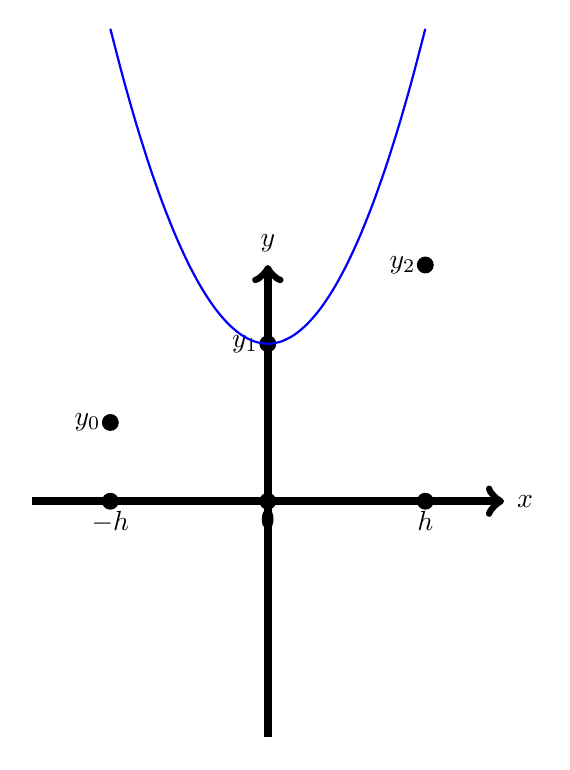
\begin{tikzpicture}
    % Koordinat eksenlerini çiz
    \draw[line width=1mm,->] (-3,0) -- (3,0) node[right] {$x$}; % x eksen
    \draw[line width=1mm,->] (0,-3) -- (0,3) node[above] {$y$}; % y eksen

    % x eksenindeki noktalar
    \draw[fill=black] (-2,0) circle (0.1) node[below] {$-h$};
    \draw[fill=black] (0,0) circle (0.1) node[below] {$0$};
    \draw[fill=black] (2,0) circle (0.1) node[below] {$h$};

    % y eksenindeki noktalar
    \draw[fill=black] (-2,1) circle (0.1) node[left] {$y_0$};
    \draw[fill=black] (0,2) circle (0.1) node[left] {$y_1$};
    \draw[fill=black] (2,3) circle (0.1) node[left] {$y_2$};

    % Parabolü çiz
    \draw[domain=-2:2, smooth, variable=\x, blue, thick] plot ({\x}, {\x*\x + 2});
\end{tikzpicture}
\end{center}

\section{Koordinat düzlemi üzerinde yer alacak h ve y değerleri belirlenir.}
$h = paramH$\\
$y = paramY$

\section{Polinomlar için x - h dönüşü yapılır.}
paramXToH


\section{Katsayılardan oluşan sembolik matris oluşturulur.}
\begin{center}
$\begin{bmatrix}
prmSymbolicMatrix
\end{bmatrix} $
\end{center}

\section{İndirgenmiş eşelon matrisin oluşturulması için katsayılardan oluşan başlangıç matrisi oluşturulur.}
\begin{center}
$\begin{bmatrix}
1&-1&1&y_{-1}\\
0&0&1&y_{0}\\
1&-1&1&y_{1}\\
\end{bmatrix} $
\end{center}

\section{Adım adım indirgenmiş matris hesaplanır.}
\begin{center}
$PivotRow= 0, Pivot: 0, (R3 \leftarrow R3 + R1 * -1) $\\
$\begin{bmatrix}
1&-1&1&y_{-1}\\
0&0&1&y_{0}\\
1&-1&1&y_{1}\\
\end{bmatrix} $
\end{center}

\section{İndirgenmiş eşelon matris}
\begin{center}
$\begin{bmatrix}
1&0&0&((y_{-1}) + ((y_{1} - (y_{-1})) * 0.5)) - y_{0}\\
0&1&0&(y_{1} - (y_{-1})) * 0.5\\
0&-0&1&y_{0}\\
\end{bmatrix} $
\end{center}


\end{document}
